\documentclass[11pt,oneside]{article}

\usepackage{clrscode3e}
\usepackage{amsmath}
\usepackage{amssymb}
\usepackage{enumerate}
\usepackage{hyperref}
\hypersetup{
  pdfborder = {0 0 0}
  pdfauthor = {Erik Helin, Jim Holmstr\"{o}m},
  pdfkeywords = {avalg11, tsp},
  pdftitle = {Project TSP report},
  pdfsubject = {Project TSP report},
  pdfpagemode = UseNone
}
\usepackage{tikz}

\newcommand{\email}[1]{\href{mailto:#1}{\texttt{#1}}}

\begin{document}
\title{Report for project TSP, DD2440}
\author{Erik Helin \\ \email{ehelin@kth.se} \and 
        Jim Holmstr\"{o}m \\ \email{jimh@kth.se}}
\maketitle

\begin{abstract}
    This report desribes the implementation of an algorithm that factors integers 
into prime factors. Factoring an integer into prime factors means finding a
representation of an integer $n = p_1^{k_1}p_2^{k_2} \ldots p_n^{k_n}$ where
$p_i$ are primes and $k_i$ are integers.
Three different algorithms were tried (separately and combined): trial
division, Pollard's $\rho$ algorithm and perfect power factorization. Pollard's
$\rho$ algorithm was tried with two different cycle detection algorithms.
The algorithms where then benchmarked using 100 random integers. 
The report concludes
that using Pollard's $\rho$ algorithm with Floyd's cycle detection resulted in
the best performance.

\end{abstract}

\clearpage
\tableofcontents
\clearpage

\section{Introduction}
\label{sec:introduction}
The factoring project is about factoring integers into prime factors. That is,
for a given number $n \in \mathbb{Z}$, $n$ can be represented as 
$n = p_1^{k_1}p_2^{k_2} \ldots p_m^{k_m}$ where $p_i$ are prime numbers and
$k_i$ are integers. The task of the project is to find these prime numbers
$p_i$ and their exponents $k_i$. As an example, $20 = 2^2 \cdot 5^1$.

Today, there is no known (non-quantum) algorithm that effectively factors very 
large integers. 
In 2010, a group of researches managed to factor a number represented by
232 bits, but this took 2 years using hundreds of machines~\cite{rsa}.

This report will describe the implementation of an algorithm for factoring
integers. Section \ref{sec:problem_statement} states the exact problem
defintion, then section \ref{sec:implementation} describes the various
algorithms being tried. In section \ref{sec:results}, these algorithms
are benchmarked and the results are then analyzed in section \ref{sec:analysis}.


\section{Problem statement}
\label{sec:problem_statement}
Given 100 unknown integers, compute and print the prime number factorization 
for each integer. If number $n_i = p_1^{k_1}p_2^{k_2} \ldots p_m^{k_m}$, then
the program should print the following on \texttt{stdout}.
\begin{align*}
&\left.\begin{aligned}
      &p_1 \\
      &p_1 \\
      &\vdots \\
      &p_1 
      \end{aligned}
\right\}
\qquad k_1 \text{ times} \\
&\left.\begin{aligned}
      &p_2 \\
      &p_2 \\
      &\vdots \\
      &p_2 
      \end{aligned}
\right\}
\qquad k_2 \text{ times} \\
&\vdots \\
&\left.\begin{aligned}
      &p_m \\
      &p_m \\
      &\vdots \\
      &p_m 
      \end{aligned}
\right\}
\qquad k_m \text{ times}
\end{align*}

The time limit for the program is 15 seconds. The text \texttt{fail} must be
printed on \texttt{stdout} if the program fails to factor a number. 
The performance of the program is measured in how many numbers the program are
able to factor within the time limit. The program must print either the correct
prime factorization or \texttt{fail} for each of the 100 numbers.

The program is \emph{not} allowed to use the \texttt{time} system call.


\section{Implementation}
\label{sec:implementation}
The TSP can be divided into two parts, constructing an initial path and
optimizing the constructed path. The section \ref{sec:constructing_the_path}
discusses various heuristics used for constructing the path and section
\ref{sec:optimizing_the_path} describes heuristics for optimzing that path.  

For all the heuristics, it is easier to view the TSP as a graph problem.
The TSP can be viewed as a graph problem, where each point $(x, y)$ is a node in
the graph, and there is an undirected edge from each point to all other points. 
The weight of each edge is the distance between the two end-points of the edge.
The TSP then reduces to find a tour that visits each node exactly once with the
minimum total edge weight.

\subsection{Constructing the path}
\label{sec:constructing_the_path}
This section will describe two different heuristics for constructing an
initial path.

\subsubsection{Nearest neighbour}
\label{sec:nearest_neighbour}
\paragraph{Heuristic}
\begin{codebox}
\Procname{$\proc{Nearest-Neighbour}(\id{cities})$}
\li $\id{visited} \gets \proc{Array}(n)$
\li \For $i \gets 0$ \To $n$
\li     \Do
            $\id{visited}[i] \gets \const{false}$
        \End
\li $\id{path} \gets \proc{Vector}()$
\li $\id{city} \gets 0$
\li \While $\proc{Size}(visited) < \proc{Size}(\id{cities})$
\label{li:nn:outer}
\li     \Do
            $\id{visited}[city] \gets \const{true}$
\li         $\proc{Append}(\id{path}, \id{city})$
\li         $min \gets \infty$
\li         $next \gets -1$
\li         \For $i \gets 0$ \To $\proc{Size}(cities)$ \label{li:nn:inner}
\li             \Do
                    \If $\proc{Distance}(\id{city}, i) < min$ and
                        $\id{visited}[i] \isequal \const{false}$
\li                     \Then
                            $min \gets \proc{Distance}(\id{city}, i)$
\li                         $next \gets i$
                        \End
                \End
\li         $city \gets next$
        \End
\li \Return $\id{path}$
\end{codebox}
\paragraph{Description} \proc{Nearest-Neighbour} simply starts at the first 
city, then repeatedly selects the closes city until all cities have been
visited. To keep track of which of the cities that have been visited,
\proc{Nearest-Neighbour} stores all the visited cities in a set.
\paragraph{Running time}
Let $n$ be the number of cities to visit. The while loop on line
\ref{li:nn:outer} will then run $n$ times, since one city is added to set
\id{visited} each time. The loop on line \ref{li:nn:inner} will run $n$ times,
since it iterates over all the cities. The \proc{Distance} operation have
running time $O(1)$, so the running time of the inner loops body is $O(1)$.
Therefore, the running time of the outer loops body is $O(n)$ and the total
running time is $O(n^2)$.
\paragraph{Length of path}
Let $n$ be the number of cities, $opt$ be the optimal path for visiting the $n$
cities and $nn$ be the path
found by \proc{Nearest-Neighbour}. The relation between $opt$ and $nn$ is then
\[\frac{nn}{opt} \leq \frac{1}{2}(\lceil \log_2(n) \rceil + 1)\]
according to~\cite{johnson}. This means that for some instances, the path found
by \proc{Nearest-Neighbour} will be a factor 
$\frac{1}{2}(\lceil \log_2(n) \rceil + 1)$ larger than the optimal path.

\clearpage

\subsubsection{Greedy}
\paragraph{Heuristic}
\begin{codebox}
\Procname{$\proc{Greedy}(cities)$}
\li $n \gets \proc{Size}(cities)$
\li $deg = \proc{Array}(n, 0)$ \Comment Every element initialized to 0
\li $h = \proc{Min-Heap}()$
\li \For $i \gets 0$ \To $n$
\li     \Do
            \For $j \gets 0$ \To $n$
\li             \Do
                    $d \gets \proc{Distance}(i,j)$
\li                 $\proc{Insert}(h, (d, i, j))$ \Comment Sorted by $d$
                \End
        \End
\li $edges \gets \proc{Vector}()$
\li \While $\proc{Size}(edges) < n$ \label{li:greedy:while}
\li     \Do
            $(d, i, j) = \proc{Heap-Extract-Min}(h)$
\li         \If $deg[i] < 2$ and $((\proc{Size}(edges) \isequal (n-1)$ and
                $deg[j] \isequal 1)$ or $deg[j] \isequal 0)$
\li             \Then
                    $\proc{Append}(edges, (i, j))$
\li                 $deg[i] \gets deg[i] + 1$
\li                 $\id{in-path}[i] \gets \const{true}$
\li                 $deg[j] \gets deg[j] + 1$
\li                 $\id{in-path}[j] \gets \const{true}$
\li             \Else \textbf{continue}
                \End
        \End
\li $path \gets \proc{Vector}()$
\li $last \gets edges[0]$
\li $\proc{Append}(path, \attrib{last}{to})$
\li \While $\proc{Size}(path) < n$
\li     \Do
            \For $e \in edges$
\li             \Do
                    \If $\attrib{last}{to} \isequal \attrib{e}{from}$
\li                     \Then
                            $\proc{Append}(path, \attrib{e}{to})$
\li                         $last \gets e$
\li                         \textbf{break}
                        \End
                \End
        \End
\li \Return $path$
\end{codebox}
\paragraph{Description} \proc{Greedy} is very similar to
\proc{Nearest-Neighbour}, but instead of choosing the closest city to move to,
\proc{Greedy} always chooses the shortest edge in the graph (under some
constraints). In order for \proc{Greedy} to form a complete tour of all the
edges, the edges has to be chosen in a certain way. When a new edge is added to
the tour, the degree of the nodes at the ends of the edge must have a degree of
either 0 or 1. This is because a tour is only allowed to visit each city
\emph{exactly} once, which means one edge going in to the city and one edge
leaving the city, yielding a degree of 2.

Furthermore, when an edge gets added to tour, care must be taken to ensure that
edge does not create a cycle in the graph. This is done by checking if the city
that the edge is going to hasn't already been visited (the degree of the city
is then 0).

\paragraph{Running time}
Let $n$ be the number of cities, then there will $n^2$ edges in the
corresponding graph, because there is an edge between every city.
Inserting an element into a heap takes $O(\log(n))$, where $n$ is the size of
the heap. Since the heap $h$ will have all edges, that is $n^2$, the
\proc{Insert} operation takes $O(\log(n^2)) = O(2\log(n)) = O(\log(n))$.
Therefore, inserting all the edges into the heap will haver running time
$O(n^2\log(n))$. 

The while loop at line \ref{li:greedy:while} in
\proc{Greedy} must in the worst case run $n^2$ times, since it's not certain
that an edge gets added in each round. The body of the while loop performs
only constant-time operations except for \proc{Heap-Extract-Min} which have
running time $O(\log(n^2)) = O(\log(n))$. Therefore, the total running time of
the loop is $O(n^2\log(n))$.

The running time of the last for loop is $O(n)$, since at each round, one city
will be added to the path. This is because in city have one outgoing and one
incoming edge, since they form a tour. The body of the loop will have running
time $O(n)$, since in iterates over all edges. Therefore,
the total running time of the last for loop is $O(n^2)$.

Hence, the total running time of \proc{Greedy} is $O(n^2\log(n))$.

\paragraph{Length of path}
Let $n$ be the number of cities, $opt$ be the optimal path for visiting the $n$
cities and $g$ be the path
found by \proc{Greedy}. The relation between $opt$ and $g$ is then
\[\frac{g}{opt} \leq \frac{1}{2}(\lceil \log_2(n) \rceil + 1)\]
according to~\cite{johnson}. 

Hence, \proc{Greedy} and \proc{Nearest-Neighbour} performs equally bad in the
worst case.

\subsection{Optimizing the path}
\label{sec:optimizing_the_path}
The following algorithms are performs \emph{local} optimizations. That is, the
take an already constructed path, then make a small local change which renders
the length of the path shorter.

\subsubsection{2-opt}
\label{sec:2-opt}
\paragraph{Heuristic}
\begin{codebox}
\Procname{$\proc{Swap}(path, a, b)$}
\li $c \gets \attrib{a}{next}$
\li $d \gets \attrib{b}{next}$
\li $\attrib{c}{prev} \gets d$ 
\li $\attrib{a}{next} \gets b$
\li $\attrib{d}{prev} \gets c$ 
\li $current \gets b$
\li $prev \gets a$
\li \While $current \neq d$
\li     \Do
            $\attrib{current}{next} \gets \attrib{current}{prev}$
\li         $\attrib{current}{prev} \gets \attrib{current}{prev}$
\li         $prev \gets current$
\li         $current \gets \attrib{current}{next}$ 
        \End
\end{codebox}
\begin{codebox}
\Procname{$\proc{2-opt}(path)$}
\li $n \gets \proc{Size}(path)$
\li $\id{improvement} \gets \id{true}$
\li \While $\id{improvement} \isequal \const{true}$
\li     \Do
            $\id{improvement} \gets \const{false}$
\li         $a \gets \proc{First}(path)$
\li         $a_n \gets \attrib{a}{next}$
\li         \For $i \gets 0$ \To $n$
\li             \Do
                    $b \gets \proc{First}(path)$    
\li                 $b_n \gets \attrib{b}{next}$
\li                 \For $j \gets 0$ \To $n$
\li                     \Do
                            \If $a \neq b$ and
                                $a_n \neq b$ and
                                $b_n \neq a$ \label{li:2opt:c1}
\li                             \Then
                                    $e_1 \gets \proc{Distance}(a, a_n) +
                                               \proc{Distance}(b, b_n)$
\li                                 $e_2 \gets \proc{Distance}(a, b) +
                                               \proc{Distance}(a_n, b_n)$
\li                                 \If $e_1 > e_2$ \label{li:2opt:c2}
\li                                     \Then
                                            $\proc{Swap}(path, a, b)$
\li                                         $a_n \gets \attrib{a}{next}$
\li                                         $b_n \gets \attrib{b}{next}$
\li                                         $\id{improvement} \gets
                                             \const{true}$
                                        \End
                                \End
\li                     $b \gets \attrib{b}{next}$
\li                     $b_n \gets \attrib{b_n}{next}$
                        \End
\li             $a \gets \attrib{a}{next}$
\li             $a_n \gets \attrib{a_n}{next}$
                \End
        \End
\end{codebox}

\paragraph{Description}
The idea behind \proc{2-opt} is to traverse the constructed tour and checking
if two edges can be swapped to yield a shorter tour.
\begin{figure}[ht!]
    \centering
    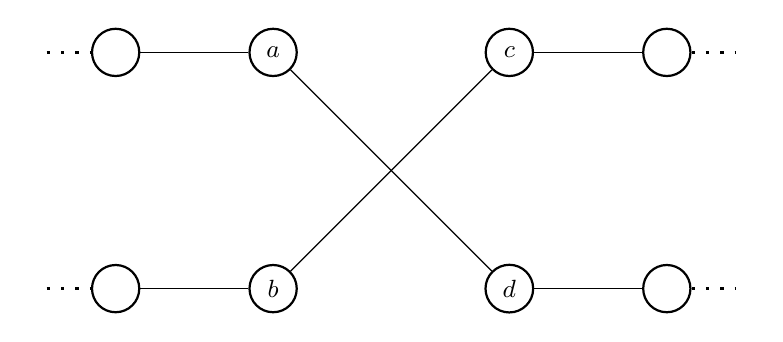
\begin{tikzpicture}
        [ele/.style = {circle, draw, thick, minimum size=6mm,
        font=\small}]
        \node (e2) at (-1, 3) {};
        \node (e3) at (-1, 0) {};
        \node[ele] (e0) at (0,3) {}; 
        \node[ele] (a) at (2, 3) {$a$};
        \node[ele] (c) at (5, 3) {$c$};
        \node[ele] (e1) at (0,0) {}; 
        \node[ele] (b) at (2, 0) {$b$};
        \node[ele] (d) at (5, 0) {$d$};
        \node[ele] (e4) at (7,3) {}; 
        \node[ele] (e5) at (7,0) {}; 
        \node (e6) at (8, 3) {};
        \node (e7) at (8, 0) {};

        \draw[-, loosely dotted, very thick] (e2) -- (e0);
        \draw[-, loosely dotted, very thick] (e3) -- (e1);
        \draw[-, loosely dotted, very thick] (e5) -- (e7);
        \draw[-, loosely dotted, very thick] (e4) -- (e6);
        \draw (e0) -- (a); 
        \draw (e1) -- (b); 
        \draw (a) -- (d); 
        \draw (b) -- (c); 
        \draw (c) -- (e4); 
        \draw (d) -- (e5); 
    \end{tikzpicture}
    \caption{A path before the swap made by \proc{2-opt}}
    \label{fig:2opt:pre}
\end{figure}
\begin{figure}[ht!]
    \centering
    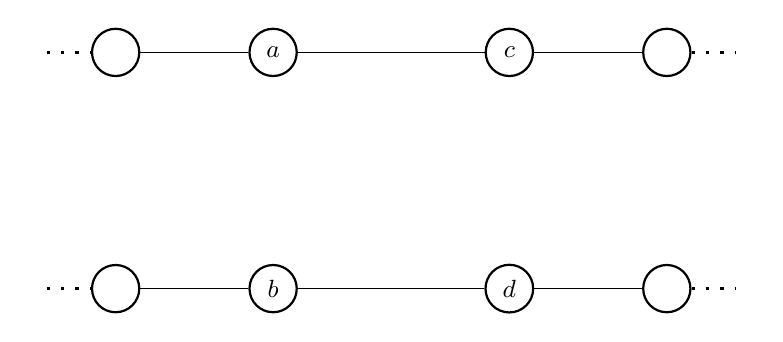
\begin{tikzpicture}
        [ele/.style = {circle, draw, thick, minimum size=6mm,
        font=\small}]
        \node (e2) at (-1, 3) {};
        \node (e3) at (-1, 0) {};
        \node[ele] (e0) at (0,3) {}; 
        \node[ele] (a) at (2, 3) {$a$};
        \node[ele] (c) at (5, 3) {$c$};
        \node[ele] (e1) at (0,0) {}; 
        \node[ele] (b) at (2, 0) {$b$};
        \node[ele] (d) at (5, 0) {$d$};
        \node[ele] (e4) at (7,3) {}; 
        \node[ele] (e5) at (7,0) {}; 
        \node (e6) at (8, 3) {};
        \node (e7) at (8, 0) {};

        \draw[-, loosely dotted, very thick] (e2) -- (e0);
        \draw[-, loosely dotted, very thick] (e3) -- (e1);
        \draw[-, loosely dotted, very thick] (e5) -- (e7);
        \draw[-, loosely dotted, very thick] (e4) -- (e6);
        \draw (e0) -- (a); 
        \draw (e1) -- (b); 
        \draw (a) -- (c); 
        \draw (b) -- (d); 
        \draw (c) -- (e4); 
        \draw (d) -- (e5); 
    \end{tikzpicture}
    \caption{A path after the swap made by \proc{2-opt}}
    \label{fig:2opt:post}
\end{figure}
The idea can be seen in figure \ref{fig:2opt:pre} and figure
\ref{fig:2opt:post}. Therefore, \proc{2-opt} iterates through all possible
quartets ($a$, $a_n$, $b$, $b_n$) of cities and checks if the edges should be
swapped. Any two edges should \emph{not} be swapped in they share a common
node and any two edges should only be swapped if the swap reduces the length of
the path. This is checked by line \ref{li:2opt:c1} and \ref{li:2opt:c1} in
\proc{2-opt}.

Since our implementation of \proc{2-opt} uses a double linked list,
\proc{Swap} needs to ensure that edges between all nodes are correct. When
swapping two edges in double linked list, the list has to be iterated over to 
update all the nodes so their $prev$ and $next$ pointers are consistent.

\paragraph{Running time}
The running time for \proc{Swap} is clearly $O(n)$, since in the worst case,
all edges in the list have to be corrected. The inner for loop in \proc{2-opt}
is run $n$ times, and the body consists only of operations of running time
$O(1)$ and \proc{Swap} operation of running time $O(n)$. Therefore, the total
running time of the inner for loop $O(n^2)$. The outer for loops in being run
$n$ times, and the body of the outer for loop only performs operations with
running time $O(1)$ except for the inner for loop. Therefore, the running time
of the outer for loop is $O(n^3)$.

The question, how many iterations does \proc{2-opt} need before it has
optimized the given path? In the worst case, \proc{2-opt} needs
$\Theta(2^{n/2})$ iterations before finding a local optimal
solution~\cite{johnson}. However, in practice, the number of iterations needed
are usually $\Theta(n)$~\cite{hastad}, which results in total running time of
$O(n^4)$ for this implementation of \proc{2-opt}.

\subsection{Implementation of algorithms}
\label{sec:implementation_of_algorithms}
All heuristics were implemented in the C++ programming language. Of the
heuristics described, \proc{Nearest-Neighbour} and \proc{2-opt} were
implemented.

\subsubsection{Implementation of \proc{Distance}}
The \proc{Distance} was implemented by calculating all the distances between
all cities and storing the results in a matrix. A call to \proc{Distance} with
arguments $(i, j)$ then simply returned the value of the $i$:th row and the
$j$:th column in the matrix.

\subsubsection{Implementing \proc{Nearest-Neighbour}}
The \proc{Nearest-Neighbour} heuristic was implemented identically to the 
pseudo-code described in section \ref{sec:nearest_neighbour}.

\subsubsection{Implementing \proc{2-opt}}
\label{sec:implementing_2-opt}
The \proc{2-opt} heuristic was also implemented similar to the pseudo-code in
\ref{sec:2-opt}. One detail, which isn't noticeable in the pseudo code, was the
implementation of the double linked list. Since the size of the list is always
known beforehand, all memory that was needed for the list was allocated in the
constructor, instead of allocating a new element of the linked list each time
an element was appended. Then, each insertion of a new element was done 
in-place in the allocated array.

When implementing \proc{2-opt}, we also used a counter to ensure that
\proc{2-opt} didn't run longer than 2 seconds.


\section{Results}
\label{sec:results}
The tests area solely based on the running time and score on the
\texttt{KATTIS}~\cite{kattis} problem \texttt{oldkattis:tsp}~\cite{kattis-tsp}

\subsection{\proc{Nearest-Neighbour}}
\begin{table}[ht!]
    \centering
    \begin{tabular}{|c|c|}
        \hline 
        \textbf{Time (s)} & \textbf{Score} \\ \hline
        0.10 & 3.00632 \\ \hline
    \end{tabular}
    \caption{Results using only the \proc{Nearest-Neighbour} heuristic}
    \label{table:nn}
\end{table}

\subsection{\proc{Nearest-Neighbour} and \proc{2-opt}}
First, the path was constructed using \proc{Nearest-Neighbour} and then it was
optimized using \proc{2-opt}. The column named counter in the table describes
the maximum value of the counter, see the last part of section
\ref{sec:implementing_2-opt} for more details.
\begin{table}[ht!]
    \centering
    \begin{tabular}{|c|c|c|}
        \hline
        \textbf{Counter} & \textbf{Time (s)} & \textbf{Score} \\ \hline
            1 &  3.1085 & 0.14 \\ \hline
            2 &  3.8379 & 0.09 \\ \hline
            3 &  4.0749 & 0.12 \\ \hline
            5 &  4.4453 & 0.14 \\ \hline
           10 &  4.8774 & 0.12 \\ \hline
           20 &  6.5306 & 0.11 \\ \hline
           30 &  7.7677 & 0.12 \\ \hline
           50 & 10.1412 & 0.10 \\ \hline
          100 & 13.2045 & 0.11 \\ \hline
          200 & 16.4654 & 0.16 \\ \hline
          300 & 18.2710 & 0.32 \\ \hline
          500 & 19.1797 & 0.38 \\ \hline
         1000 & 19.1928 & 0.39 \\ \hline
         2000 & 19.1928 & 0.38 \\ \hline
    
    \end{tabular}
    \caption{Results using \proc{Nearest-Neighbour} and \proc{2-opt}}
    \label{table:nn_and_2-opt}
\end{table}


\section{Analysis}
\label{sec:analysis}
The results from table \ref{table:miller-rabin} shows that it is good to use 
a primality test as an initial test, since one number was prime.
The running time also shows that is a fast operation.

The results in table \ref{table:trial} then shows that trial division alone 
does not suffice as an algorihtm for factoring integers. It it also worth
pointing out that there was no gain in increasing the number of primes used from
1718 to 10000. This is because the prime factors of most of the number are
larger than 10000th prime, rendering the trial division test useless.

When comparing the different implementations of Pollard's $\rho$ algorithm, one
clearly sees that in our case, Floyd's cycle detection method outperforms
Brent's cycle detection. The reason for this might be that the number used at
Kattis suits Floyd's cycle detection algorithm better (Brent's algorithm ended
up with $x = y = n$ more often that Floyd's). Due to this, we decided to use
Floyd's cycle detection. 

It is also interesting that the combined use of trial
division, perfect power factorization and Pollard's $\rho$ algorithm shows no
performance increase compated to using only Pollard's $\rho$ algorithm.
This is probably due to the fact that the numbers that trial division and
perfet power factorization can factor can also be quickly factored with
Pollard's $\rho$ algorithm. When comparing
Brent's cycle detection with and without all trial division and perfect power
hashing, the two extra algorithms did help. This further justifies the thought
that Brent's cycle deteciton is weaker than Floyd's on the number available on
Kattis. Since there were no performance gains in using trial division and
perfect power hashing with Floyd's cycle detection, we decided to remove these
two steps.

Since we didn't gain any increased results from using perfect power hashing, 
we decicded to not implement Newton's method.

When comparing the different random algorithms used when restarting Pollard's
$\rho$ algorithm, the reason that \texttt{rand} is faster is probably because
it is much simpler and doesn't deal with as large number as
\texttt{mp\_urandomm} does.

It is not surprising that the number of factored number increases as the
cut-off increases, since this gives the factoring algorithm more time. These
numbers also shows the importance of tweaking the implementation to be as fast
as possible, since a fast implementation can use a higher cut-off.


\section{Conclusion}
\label{sec:conclusion}
The final algorithm being used was Pollard's $\rho$ algorithm with Floyd's
cycle detection toghether with \texttt{rand} for generating random numbers,
since this combination achieved the highest result.

Given more time, we would have liked to invest more time in increasing the
performance of the cycle detection part of Pollard's $\rho$ algorihtm. As a
start, the
Wikipedia article~\cite{wiki:pollard} mentions some adjustments that can be
done to speed up the cycle detection.

We would also have liked to come up with a better algorithm for noticing
numbers that our algorihtm probably wouldn't be able to factor. This would have
saved us time for factoring other numbers that we might haven been able 
to factor.


\begin{thebibliography}{9}
    \bibitem{wikipedia:tsp}
Wikipedia,
\emph{Travelling Salesman Problem} \\
\url{http://en.wikipedia.org/wiki/Travelling_salesman_problem} \\
2011

\bibitem{wikipedia:euclidean_distance}
Wikipedia,
\emph{Euclidean Distance} \\
\url{http://en.wikipedia.org/wiki/Euclidean_Distance} \\
2011

\bibitem{johnson}
David S. Johnson and Lyle A. McGeoch,
\emph{The Traveling Salesman Problem: A Case Study in Local Optimization.},
in Local Seach in Combanitorial Optimization,
E. H. L Aarts and J. K. Lenstra (eds.),
John Wiley And Sons,
London,
1997,
pp 215-310

\bibitem{hastad}
Johan H\r{a}stad,
\emph{Notes for the course advanced algorithms},
January, 2000

\bibitem{kattis}
Scrool and KTH,
\emph{KATTIS-KTH} \\
\url{https://kth.kattis.scrool.se/} \\
2011

\bibitem{kattis-tsp}
KTH,
\emph{Travelling Salesperson 2D} \\
\url{https://kth.kattis.scrool.se/problems/oldkattis:tsp} \\
2011

\bibitem{wikipedia:lin}
Wikipedia,
\emph{Lin-Kernighan heuristic} \\
\url{http://en.wikipedia.org/wiki/Lin-Kernighan_heuristic} \\
2011

\bibitem{wikipedia:3-opt}
Wikipedia,
\emph{3-opt} \\
\url{http://en.wikipedia.org/wiki/3-opt} \\
2011

\bibitem{wikipedia:christofides}
Wikipedia,
\emph{Christofides algorithm} \\
\url{http://en.wikipedia.org/wiki/Christofides_algorithm} \\
2011

\end{thebibliography}

\end{document}
